% Build this document with LuaTeX, a modern Unicode-aware LaTeX engine
% that uses system TTF and OTF font files.
% This is needed for the fontspec, microtype, and nolig packages.
%
% We're using KOMA Script to hand-tune footnotes and TOC appearance.
% It should be available in your texlive distribution,
% which is how most distros package LaTeX.
\documentclass[fontsize=10pt, numbers=endperiod]{scrartcl}

% Margins: see http://practicaltypography.com/page-margins.html and
% http://practicaltypography.com/line-length.html
% We're aiming for 80-ish characters per line.
\usepackage[letterpaper, left=0.75in,right=0.75in,top=1in,bottom=1in]{geometry}

% Font specification.
% Use Equity for the body text,
% Roboto for sans serif,
% and mononoki for monospace text.
% Feel free to pick your own fonts or comment these lines out to use TeX's
% traditional Computer Modern.
\usepackage[no-math]{fontspec}
\usepackage[fleqn]{amsmath}
\setmainfont[Ligatures=TeX,
             Numbers=Lowercase,
             SmallCapsFont={Equity Caps A},
             SmallCapsFeatures={StylisticSet=10}, % Set everything in \textsc{} as small caps
             StylisticSet=01, % Slightly smaller quotes, asterisks, etc.
            ]{Equity Text A}
\setsansfont[Ligatures=TeX, Scale=MatchUppercase,
             BoldFont={* Medium},
             BoldItalicFont={* Medium Italic},
            ]{Roboto}
\setmonofont[Scale=MatchLowercase]{mononoki}

\newfontfamily{\headingface}{Equity Text B}[
             Ligatures=TeX,
             Numbers=Lowercase,
             SmallCapsFont={Equity Caps B},
             SmallCapsFeatures={StylisticSet=10}, % Set everything in \textsc{} as small caps
             StylisticSet=01, % Slightly smaller quotes, asterisks, etc.
            ]

\usepackage[italic]{mathastext}

\usepackage{polyglossia}
\setdefaultlanguage[variant=american]{english}

\usepackage{microtype} % Font expansion, protrusion, and other goodness

% Disable ligatures across grapheme boundaries
% (see the package manual for details.)
\usepackage[english]{selnolig}

% Use symbols for footnotes, resetting each page
\usepackage[perpage,bottom,symbol*]{footmisc}

% Left flush footnotes. See the KOMA Script manual.
\deffootnote[1em]{1em}{1em}{\thefootnotemark}
% Set the width of the rule separating body text and footnotes
\setfootnoterule{0.7\textwidth}

% Like many fonts, Equity's asterisk is already set in a "superscripted" form.
% Superscripting *that* makes it annoyingly small.
% To fix this, we have to redefine footnote marks so that they aren't superscript,
% then raise all the other symbols.
%
% Feel free to remove this if your body type doesn't have this peculiarity,
% but unfortunately many do.
% See http://tex.stackexchange.com/a/16241
%
% We use the Unicode symbols themselves (instead of \dagger, \ddagger, \P, etc.)
% because the latter fall back to Computer Modern/Latin Modern in some cases,
% (e.g., if you're using mathastext instead of unicode-math).
% Alternatively, you could use \textdagger, \textddagger, etc.,
% but this seems more concise.
\DefineFNsymbols*{tweaked}{%
    {*}%
    {\textsuperscript†}%
    {\textsuperscript‡}%
    {\textsuperscript{◊}}%
    {\textsuperscript{¶}}%
    {**}%
    {\textsuperscript{††}}%
    {\textsuperscript{‡‡}}%
}
\setfnsymbol{tweaked}
\deffootnotemark{\thefootnotemark}

% Use the tocstyle package to give all ToC items sans serif font.
% We also want our monospace font to match the uppercase height of the sans serif.
% (Matching x-heights make it quite small in comparison.)
% Note: tocstyle is currently in alpha, so feel free to tweak this as needed.
% At time of writing, it seems to be the simplest way to get the intended effect.
\usepackage{tocstyle}
\settocfeature{pagenumberhook}{\addfontfeature{Numbers=Tabular}}
\settocfeature{entryvskip}{2pt}

% Don't use a sans font for description labels.
\addtokomafont{descriptionlabel}{\rmfamily\mdseries}
\setkomafont{disposition}{\rmfamily}
\setkomafont{section}{\headingface\large\itshape}
\setkomafont{subsection}{\normalsize\itshape}
\renewcommand*\thesection{\upshape\arabic{section}}

% Use uppercase numbers for numbered lists.
% (We're using lowercase ones for the body text.)
% See http://tex.stackexchange.com/a/133186
\usepackage{enumitem}
\setlist[enumerate]{font=\addfontfeatures{Numbers=LowercaseOff, StylisticSet=02}}

% Custom footer
\usepackage{scrlayer-scrpage}
\setkomafont{pagefoot}{\sffamily\upshape}
\pagestyle{scrheadings}

\usepackage{minted} % Syntax highlighting via Pygments

\usepackage{graphicx}
\usepackage[font=footnotesize,justification=raggedright]{caption}

\usepackage{tikz} % Duck and cover.

\newcommand{\codesize}{\fontsize{10pt}{12pt}}

% Syntax highlighting for ARM asm (minted doesn't do this well)
\usepackage{listings}
\lstset{
basicstyle=\ttfamily\codesize\selectfont,
keywordstyle=\color{darkGreen}\bfseries,
commentstyle=\textcolor[rgb]{0.25,0.50,0.50}
}
% listings definitions for ARM assembly.
% Get them from https://github.com/frosc/arm-assembler-latex-listings,
% install as shown at http://tex.stackexchange.com/a/1138/92465
\usepackage{lstlangarm} % See above

\usepackage{multicol}
\setlength\columnsep{2em}
%\setlength\parskip{0em}
\setlength\parindent{1.5em}

\title{What every systems programmer should know about lockless concurrency}
\author{Matt Kline}
\date{November 21, 2017}

% Custom footer
% Hyperlinks
\usepackage[unicode,pdfusetitle]{hyperref}
\usepackage{xcolor}
\definecolor{darkGreen}{HTML}{008000}
\hypersetup{
    colorlinks=true, % Use colors
    linkcolor=violet, % Intra-doc links
    urlcolor=blue % URLs are blue
}

% See http://tex.stackexchange.com/a/68310
\makeatletter
\let\runauthor\@author
\let\rundate\@date
\let\runtitle\@title
\makeatother

% Spend a bit more time to get better word spacing.
% See http://tex.stackexchange.com/a/52855
\emergencystretch=1em

% Use \punckern to overlap periods, commas, and footnote markers
% for a tighter look.
% Care should be taken to not make it too tight - f" and the like can overlap
% if you're not careful.
\newcommand{\punckern}{\kern-0.4ex}
% For placing commas close to, or under, quotes they follow.
% We're programmers, and we blatantly disregard American typographical norms
% to put the quotes inside, but we can at least make it look a bit nicer.
\newcommand{\quotekern}{\kern-0.5ex}


% Create an unbreakable string of text in a monospaced font.
% Useful for `command --line --args`
\newcommand{\monobox}[1]{\mbox{\texttt{#1}}}

\newcommand{\keyword}[1]{\monobox{\color{darkGreen}#1}}

% C++ looks nicer if the ++ is in a monospace font and raised a bit.
% Also, use uppercase numbers to match the capital C.
\newcommand{\cpp}[1]{C\kern-0.1ex\raisebox{0.15ex}{\texttt{++}}{\addfontfeature{Numbers=LowercaseOff}#1}}
\newcommand{\clang}[1]{C{\addfontfeature{Numbers=LowercaseOff}#1}}
\newcommand{\csharp}{C\raisebox{0.25ex}{\#}}

\newcommand{\fig}[1]{Figure~\ref{#1}}

% Italicize new terms
\newcommand{\introduce}[1]{\textit{#1}}

\newcommand{\secref}[1]{\hyperref[#1]{\textsc{\S}\ref*{#1}}}

% Feel free to futz with the spacing above and below these.
% (Given the number of code snippets and figures,
% they can really make or break the spacing of the paragraphs.
% Keep in mind that TeX only lays out a page at a time,
% so you need to more or less look at how each page is individually handled.
\newenvironment{colfigure}
  {\par\vspace{1\baselineskip minus 0.5\baselineskip}\noindent\minipage{\linewidth}}
  {\endminipage\vspace*{1\baselineskip minus 0.7\baselineskip}}

% Spend a bit more time to get better word spacing.
% See http://tex.stackexchange.com/a/52855/92465
\emergencystretch=1em

% Try harder not to screw up footnotes in multicols environments.
% See the multicol manual.
%\setcounter{collectmore}{-2}

\begin{document}
% Custom title instead of \maketitle
\begin{center}
\sffamily\Large \textbf{\runtitle}
\bigskip

\normalsize
\runauthor
\smallskip

\rundate
\end{center}
\bigskip

\begin{center}\begin{minipage}{0.7\linewidth}
\begin{center}
\large \bfseries\itshape Abstract
\end{center}

Seasoned programmers are familiar with concurrency
tools like mutexes, semaphores, and condition variables.
But what makes them work?
How do we write concurrent code when we can't use them,
like when we're working below the operating system in an embedded environment,
or when we can't block due to hard time constraints?
And since your system transforms your code into things you didn't write,
running in orders you never asked for, how do multithreaded programs work at all?
Concurrency---especially on modern hardware---is a complicated and unintuitive
topic, but let's try to cover some fundamentals.
\bigskip

\tableofcontents
\end{minipage}\end{center}
\medskip

\begin{multicols*}{2}
\section{Background}
\label{background}

Modern computers run several instruction sequences concurrently.
We call them different names depending on the context---processes, threads, tasks,
interrupt service routines, and so on---but many of the same principles apply
across the board.
On single-core machines, these sequences take turns,
sharing the \textsc{cpu} in short slices of time.
On multiprocessors, several can run in parallel, each on its own core.

While computer scientists have invented many useful abstractions,
these instruction streams (let's call them \emph{threads} from here on out for
the sake of brevity) ultimately interact with one another by sharing bits of state.
For this to work, we must be able to reason about
the order of the reads and writes communicating threads make to memory.
Consider a simple example where thread \textit{A} shares
an integer with others.
It writes the value to some variable,
then sets a flag to instruct other threads to read whatever it just stored.
As code, this might resemble:
\begin{colfigure}
\begin{minted}[fontsize=\codesize]{cpp}
int v;
bool v_ready = false;

void threadA()
{
  // Write the value
  // and set its ready flag.
  v = 42;
  v_ready = true;
}
\end{minted}
\end{colfigure}
\begin{colfigure}
\begin{minted}[fontsize=\codesize]{cpp}
void threadB()
{
  // Await a value change and read it.
  while (!v_ready) { /* spin */ }
  const int my_v = v;
  // Do something with my_v...
}
\end{minted}
\end{colfigure}
Our system must guarantee that other threads observe \textit{A's} write to
\texttt{v\_ready}
only \emph{after A's} write to \texttt{v}.
(If another thread can ``see'' \texttt{v\_ready} change before it sees \texttt{v}
change, our communication scheme can't work.)

This appears to be an incredibly simple guarantee to provide,
but nothing is as it seems.
For starters, any compiler worth its salt will
happily modify and reorder your code to take better advantage of the hardware
it runs on.
So long as the resulting instructions run to the same effect
\emph{for the current thread,}
reads and writes can be moved to avoid pipeline stalls\footnote{%
Most \textsc{cpu} designs execute parts of several instructions in parallel
to increase their clock speed (see \fig{pipeline}).
When the result of an instruction is needed by
another instruction in the pipeline, the \textsc{cpu} may need
to suspend forward progress, or \introduce{stall,} until that result is ready.}
or to improve locality.\punckern\footnote{%
\textsc{ram} is not read in single bytes, but in chunks called cache lines.
If variables that are used together can be placed on the same cache line,
several can be read or written at once.
(We'll discuss caches and memory hierarchies shortly.)}
Variables can be assigned to the same memory location if they're never used
in overlapping time frames.
Instructions can be executed speculatively, before a branch is taken,
then undone if the compiler guessed incorrectly.\punckern\footnote{This is
especially common when using profile-guided optimization.}
%(These sorts of optimizations  sometimes called the ``as-if'' rule in \cpp{}.)

Even if we used a compiler that didn't reorder our code,
we'd still in trouble, since our hardware does it too!
Modern \textsc{cpu} designs handle incoming instructions in
a \emph{much} more complicated fashion than traditional pipelined approaches
like the one shown in \fig{pipeline}.
They contain multiple data paths, each for different types of instructions,
and schedulers which reorder and route instructions through these paths.
\begin{colfigure}
\centering
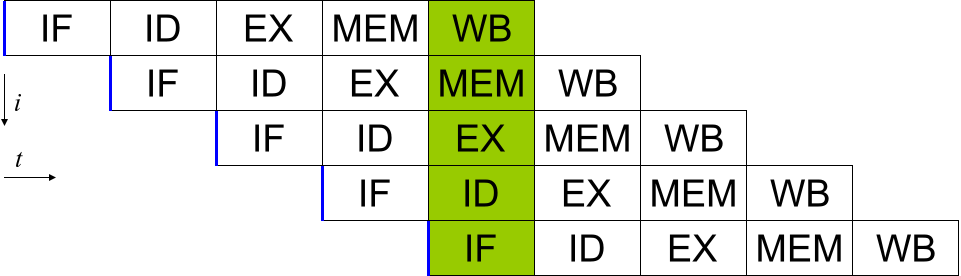
\includegraphics[keepaspectratio,width=0.7\linewidth]{pipeline}
\captionof{figure}{A traditional five-stage \textsc{cpu} pipeline
    with fetch, decode, execute, memory access, and write-back stages.
    Modern designs are much more complicated,
    often reordering instructions on the fly.
    \\ Image courtesy of
    \href{https://commons.wikimedia.org/wiki/File:Fivestagespipeline.png}{Wikipedia}.}
\label{pipeline}
\end{colfigure}

It's also easy to make naïve assumptions about how memory works.
If we imagine a multiprocessor,
we might think of something resembling \fig{ideal-machine},
where each core takes turns performing reads and writes to the system's memory.
\begin{colfigure}
\centering
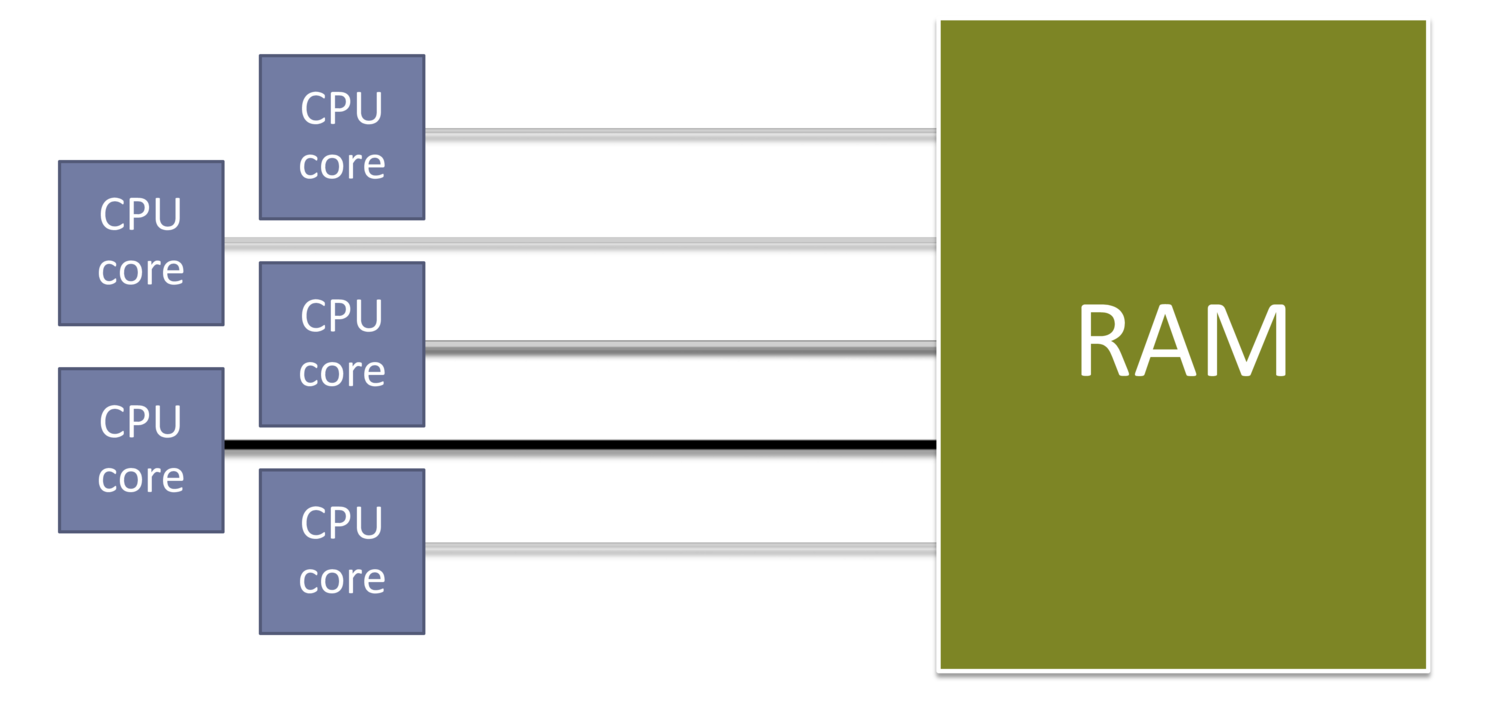
\includegraphics[keepaspectratio, width=0.8\linewidth]{ideal-machine}
\captionof{figure}{An idealized multiprocessor where cores take sequential turns
accessing a single shared set of memory.}
\label{ideal-machine}
\end{colfigure}
This is almost never the case.
While processor speeds have increased exponentially over the past decades,
\textsc{ram} hasn't been able to keep up,
creating an ever-widening gulf between the time it takes to run an
instruction and the time needed to retrieve data from main memory.
Hardware manufacturers have compensated by placing an increasing number of
hierarchical caches directly on the \textsc{cpu} die.
Each core also usually has a \introduce{store buffer} that handles
pending writes while subsequent instructions are executed.
Keeping this memory system \introduce{coherent},
so that writes made by one core are observable by others,
even if those cores use different caches,
is quite challenging.

\begin{colfigure}
\centering
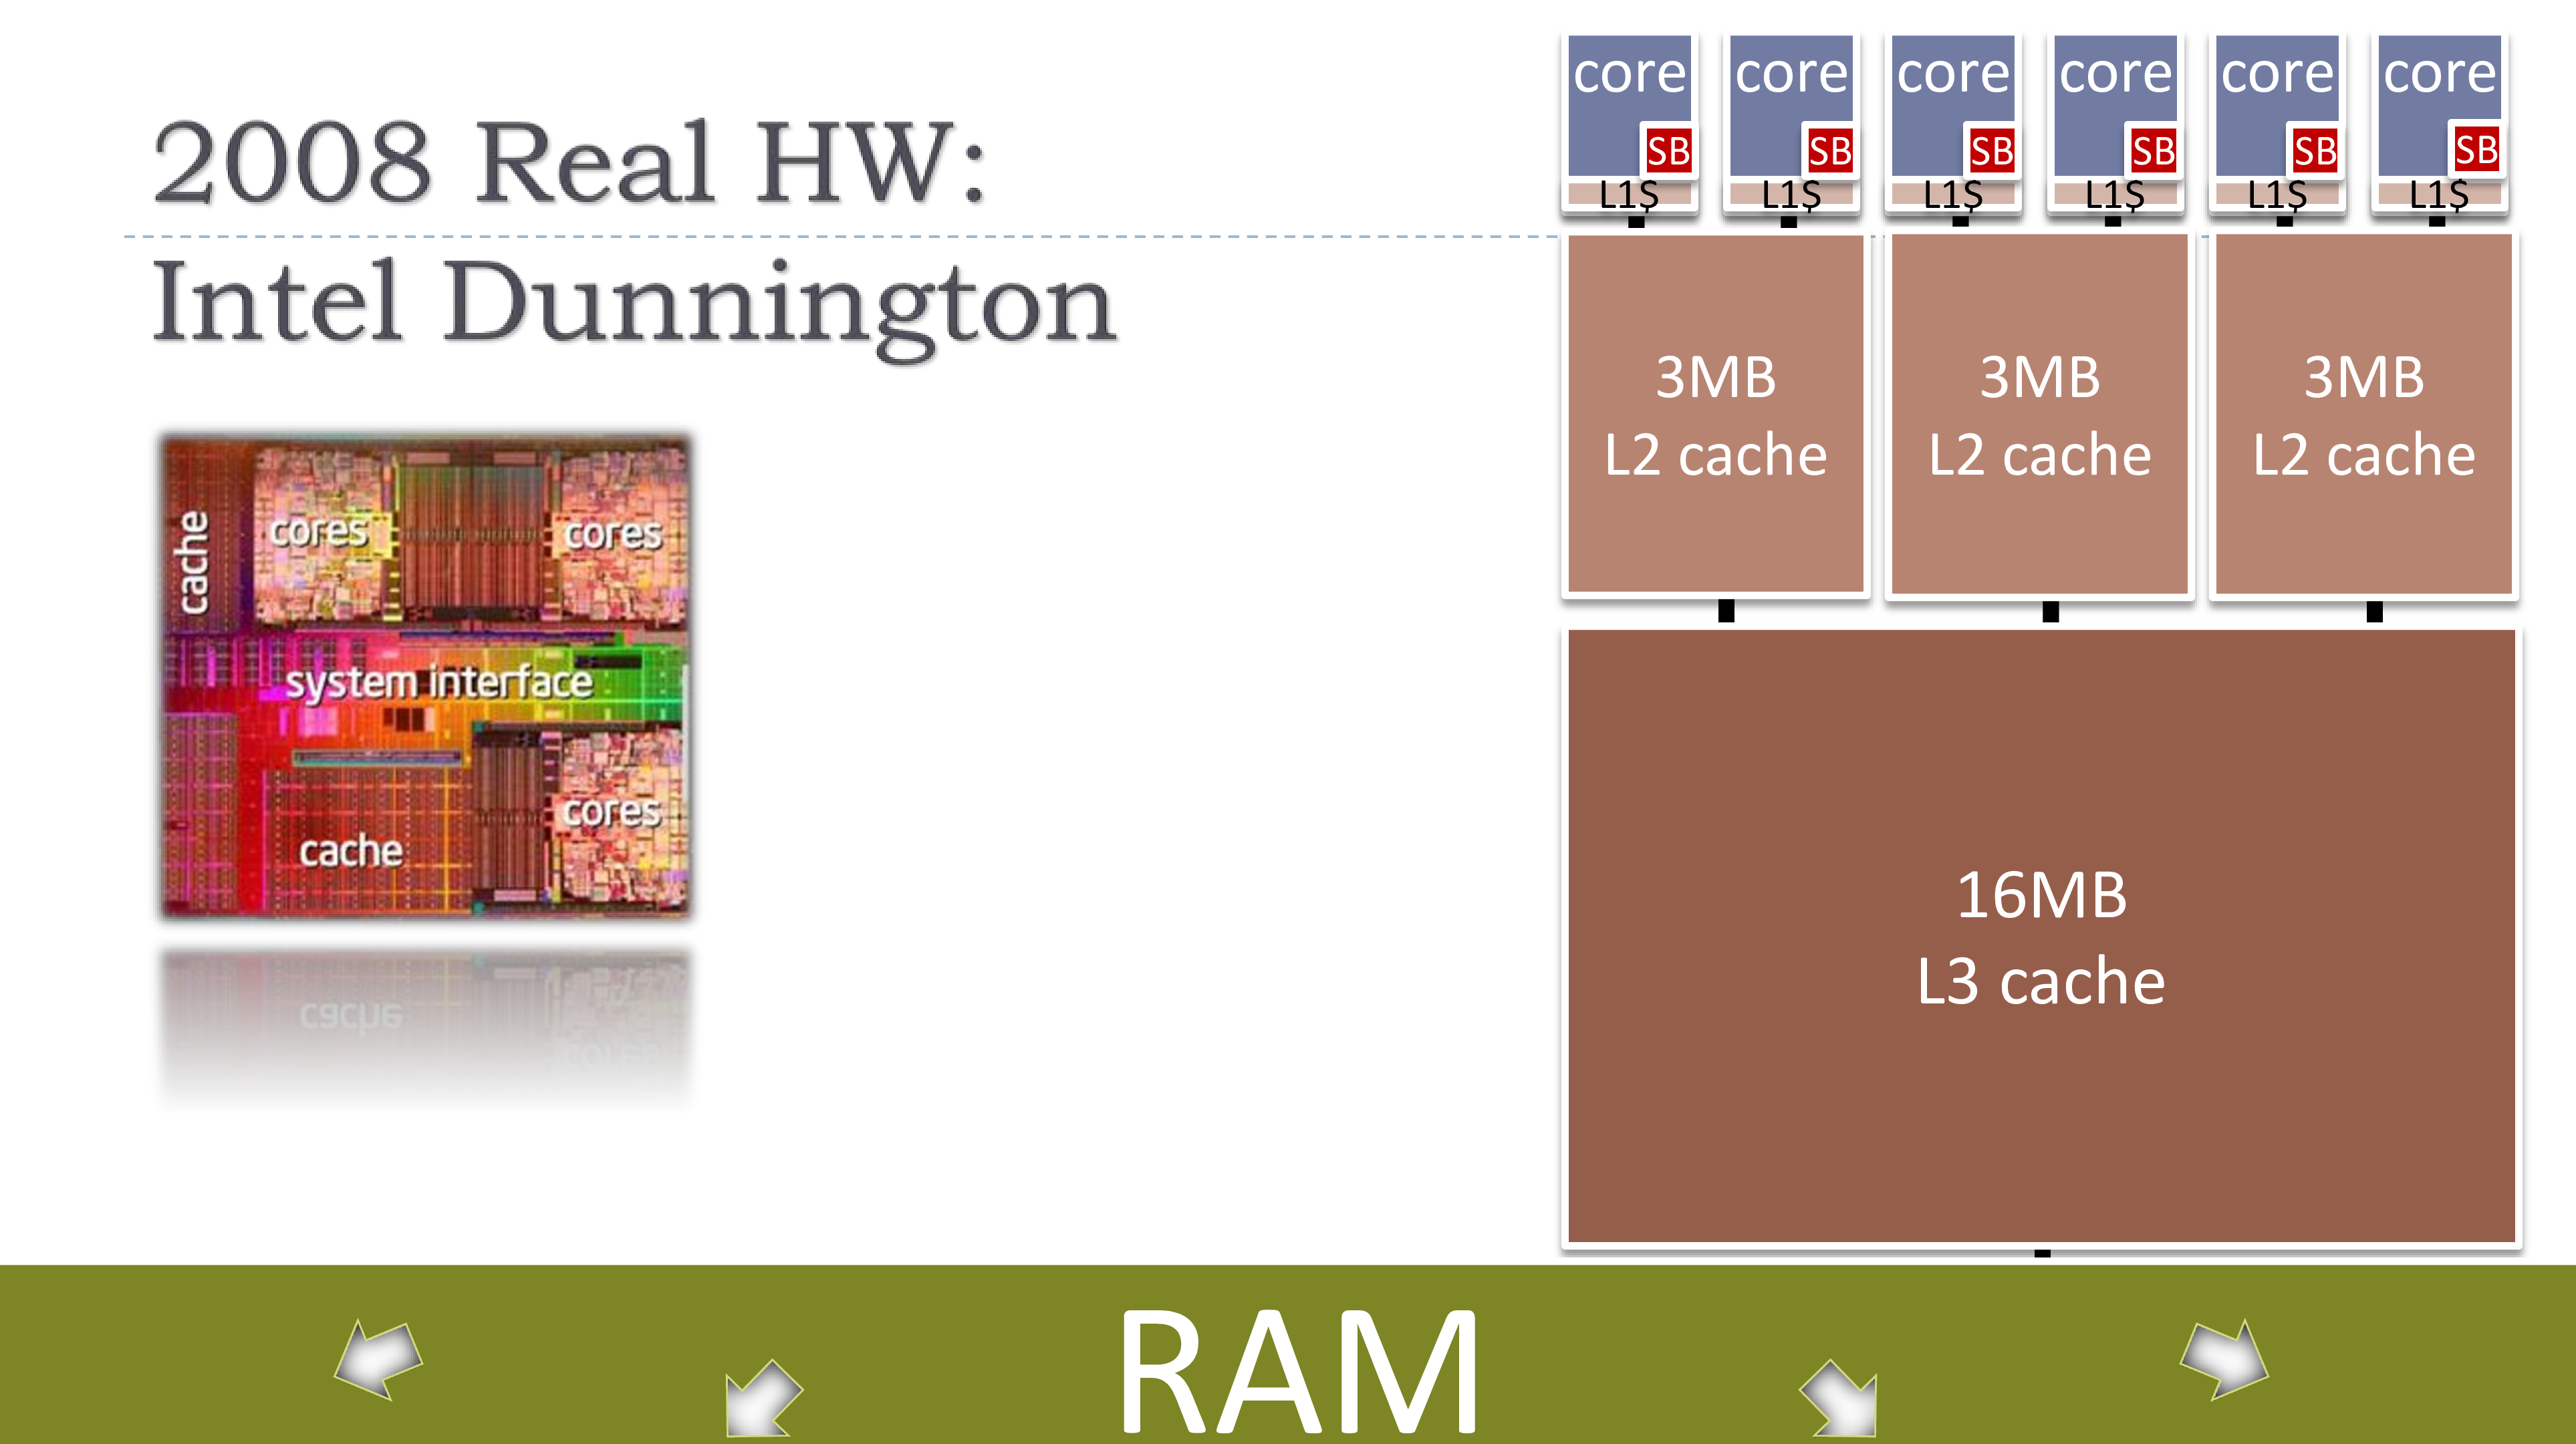
\includegraphics[keepaspectratio, width=\linewidth]{actual-machine}
\captionof{figure}{A common memory hierarchy for modern multiprocessors}
\label{dunnington}
\end{colfigure}

The net effect of these complications is that there is no consistent
concept of ``now'' in a multithreaded program,
especially one running on a multiprocessor.
Attaining some sense of order so that threads can communicate
is a team effort of hardware manufacturers, compiler writers,
language designers, and application developers.
Let's explore what we can do,
and what tools we will need.

\section{Enforcing law and order}
\label{seqcst}

Creating order in our programs requires a different approach on each
\textsc{cpu} architecture.
Until alarmingly recently, systems languages like C and \cpp{}
offered no help here,
so developers needed assembly for safe inter-thread communication.
Fortunately, the 2011 \textsc{iso} standards of both languages introduced
tools for the task.
So long as the programmer uses them correctly,
the compiler will prevent reorderings---both by the optimizer,
and by hardware---that cause data races.\punckern\footnote{The
ISO~\clang{11} standard lifted its concurrency facilities,
almost verbatim, from the \cpp{11} standard. Everything you see here
should be identical in both languages, barring some arguably cleaner syntax in
\cpp{}.}

Let's return to our example from before.
For it to work as-desired, we need to use an
\introduce{atomic type} for the ``ready'' flag:
\begin{colfigure}
\begin{minted}[fontsize=\codesize]{cpp}
int v = 0;
std::atomic_bool v_ready(false);

void threadA()
{
  v = 42;
  v_ready = true;
}
\end{minted}
\end{colfigure}
\begin{colfigure}
\begin{minted}[fontsize=\codesize]{cpp}
void threadB()
{
  while (!v_ready) { /* spin */ }
  const int my_v = v;
  // Do something with my_v...
}
\end{minted}
\end{colfigure}
The C and \cpp{} standard libraries define a series of these types
in \mintinline{c}{<stdatomic.h>} or \mintinline{cpp}{<atomic>}, respectively.
They look and act just like the integer types they mirror
(e.g., \monobox{bool}~\textrightarrow~\monobox{atomic\_bool},
\monobox{int}~\textrightarrow~\monobox{atomic\_int}, etc.),
but the compiler ensures that other loads and stores aren't reordered around
their reads and writes.
By using an atomic Boolean,
\monobox{v = 42}\, is now guaranteed to happen before
\monobox{v\_ready = true}\, in thread \textit{A},
just as \monobox{my\_v = v}\, must occur after reading \monobox{v\_ready}\,
in thread~\textit{B.}

Formally, these types provide a \textit{single total modification order}
such that,
``[\ldots] the result of any execution is the same as if the reads and writes
occurred in some order, and the operations of each individual
processor appear in this sequence in the order specified by its program.''
This model, defined by Leslie Lamport in 1979,
is called \introduce{sequential consistency}.
Informally, the important takeaway is that sequentially consistent reads
and writes act as rendezvous points for threads.
By ensuring that other operations cannot move ``past'' them,
we know that anything thread \textit{A} did before writing to an atomic
variable---such as assigning 42 to \texttt{v} before writing to
\monobox{v\_ready}---can be observed by another thread that reads the
atomic variable.

\section{Atomicity}
\label{atomicity}

Our focus so far on ordering sidestepped the other vital ingredient for
inter-thread communication: \introduce{atomicity}.
Something is atomic if it cannot be divided into smaller parts.
To see why reads and writes must have this quality to share data between threads,
let's see what problems we might encounter if they did not.

Consider a program with two threads.
One thread processes some list of files
and increments a counter each time it finishes working on one of them.
The other thread handles the user interface, and will periodically read
the counter to update a progress bar.
If that counter is a 64-bit integer, we have a problem on 32-bit machines,
since two loads or stores are needed to read or write the entire value.
If we're having a particularly unlucky time,
the first thread could be halfway through writing the counter
when the second thread reads it, receiving an incorrect value.
These unfortunate occasions are called \introduce{torn reads and writes.}

If reads and writes to shared data are atomic, however,
our problem disappears.
We can also see that, compared to the difficulties of establishing order,
ensuring atomicity is fairly straightforward:
make sure that variables used for thread synchronization are no larger than
the architecture's word size.

\section{Arbitrarily-sized “atomic” types}

Along with \texttt{atomic\_int} and friends,
\cpp{} provides the template \texttt{std::atomic<T>} for defining
arbitrary atomic types. C, lacking a similar
language feature but wanting to provide the same functionality,
added an \keyword{\_Atomic} keyword.
Running counter to what we just discussed,
\emph{any} type can be made ``atomic''\quotekern,
even if it is larger than the target architecture's word size.
In these cases, the compiler and the language runtime library automatically
surround the variable's reads and writes with locks.
For situations where this is unacceptable,\punckern\footnote{\ldots which are quite often,
since we're often using atomic operations to avoid locks in the first place.}
you can add an assertion:
\begin{colfigure}
\begin{minted}[fontsize=\codesize]{cpp}
std::atomic<Foo> bar;
ASSERT(bar.is_lock_free());
\end{minted}
\end{colfigure}
Except for there a few rare cases,\punckern\footnote{The language standards
permit atomic types to be \emph{sometimes} lock-free.
This might be necessary for architectures that
don't guarantee atomicity for unaligned reads and writes.}
the result of this check is almost always known at compile time.
Consequently, the \cpp{17} standard adds \texttt{is\_always\_lock\_free}:
\begin{colfigure}
\begin{minted}[fontsize=\codesize]{cpp}
static_assert(
  std::atomic<Foo>::is_always_lock_free);
\end{minted}
\end{colfigure}


\section{Atomic read-modify-write operations}
\label{rmw}

Loads and stores are all well and good,
but sometimes we need to read a value, modify it,
and write it back in a single atomic step.
There are a few common \introduce{read-modify-write} \textsc{(rmw)} operations.
In \cpp{}, they're represented as member functions of \texttt{std::atomic<T>}.
In \clang, they're freestanding functions.

\subsection{Exchange}
\label{exchange}

The simplest atomic \textsc{rmw} operation is an \introduce{exchange}:
the current value is read and replaced with a new one.
To see where this might be useful,
let's tweak our example from \secref{atomicity}.
Instead of displaying the total number of processed files,
we might want to show how many were processed each second.
To do so, we'll have the \textsc{ui} thread zero the counter each time it
is read.
Even if these reads and writes are atomic,
we could still run into the following race condition:
\begin{enumerate}
\item The \textsc{ui} thread reads the counter.
\item Before the \textsc{ui} thread has the chance to zero it,
    the worker thread increments it again.
\item The \textsc{ui} thread now zeroes the counter, and the previous increment
    is lost.
\end{enumerate}
If the \textsc{ui} thread exchanges the current
value of the counter with zero atomically, the race disappears.

\subsection{Test and set}

\introduce{Test-and-set} works on a Boolean value:
we read it, set it to \mintinline{cpp}{true}, and provide the value it
held beforehand.
C and \cpp{} offer a type dedicated to this purpose, called \monobox{atomic\_flag}.
We could use it to build a spinlock:
\label{spinlock}
\begin{colfigure}
\begin{minted}[fontsize=\codesize]{cpp}
std::atomic_flag af;

void lock()
{
  while (af.test_and_set()) { /* spin */ }
}

void unlock() { af.clear(); }
\end{minted}
\end{colfigure}
If the previous value is \mintinline{cpp}{false},
we are the first to acquire the lock,
and the caller can proceed with exclusive access to whatever the lock protects.
If the previous value is \mintinline{cpp}{true},
someone else has acquired the lock and we must
wait until they release it by clearing the flag.

\subsection{Fetch and…}

We can also read a value, perform some basic mathematical operation on it
(addition, subtraction, bitwise \textsc{and}, \textsc{or}, \textsc{xor}),
and return its previous value.
You might have noticed that in our exchange example,
the worker thread's additions must also be atomic,
or else we could run into a race where:
\begin{enumerate}
\item The worker thread loads the current counter value and adds one.
\item Before that thread can store the value back,
    the \textsc{ui} thread zeroes the counter.
\item The worker now performs its store, as if the counter was never cleared.
\end{enumerate}

\subsection{Compare and swap}
\label{cas}

Finally, we have \introduce{compare-and-swap} \textsc{(cas)},
sometimes called \introduce{compare-and-exchange}.
It allows us to conditionally exchange a value \emph{if} its previous value
matches some expected one.
In \clang{} and \cpp{}, \textsc{cas} resembles the following,
if it were all executed atomically:
\begin{colfigure}
\begin{minted}[fontsize=\codesize]{cpp}
template <typename T>
bool atomic<T>::compare_exchange_strong(
    T& expected, T desired)
{
  if (*this == expected) {
    *this = desired;
    return true;
  }
  else {
    expected = *this;
    return false;
  }
}
\end{minted}
\end{colfigure}

\begin{samepage}
\noindent You might be perplexed by the \texttt{\_strong} suffix.
Is there a ``weak'' \textsc{cas}?
Yes, but hold onto that thought---we'll talk about it in
\secref{spurious-ll/sc-failures}.
\end{samepage}

Let's say we have some long-running piece of work that we might want to cancel
from a \textsc{ui} thread.
We'll give it three states: \textit{idle}, \textit{running},
and \textit{cancelled}, and write a loop that exits when
it is cancelled.
\begin{colfigure}
\begin{minted}[fontsize=\codesize]{cpp}
enum class TaskState : int8_t {
  Idle, Running, Cancelled
};

std::atomic<TaskState> ts;

void taskLoop()
{
  ts = TaskState::Running;
  while (ts == TaskState::Running) {
    // Do good work.
  }
}
\end{minted}
\end{colfigure}
If we only want to set \texttt{ts} to \texttt{Cancelled} when it's
currently \texttt{Running}, but do nothing if it's already \texttt{Idle},
we could \textsc{cas}:
\begin{colfigure}
\begin{minted}[fontsize=\codesize]{cpp}

bool cancel()
{
  auto expected = TaskState::Running;
  return ts.compare_exchange_strong(
    expected, TaskState::Cancelled);
}
\end{minted}
\end{colfigure}

\section{Atomic operations as building blocks}

Atomic loads, stores, and \textsc{rmw} operations are the building
blocks for all the concurrency tools we use.
It's useful to separate them into two camps:

\introduce{Blocking} synchronization is probably the more widely-known and
understood of the two.
In this approach,
threads can be made to wait an arbitrary amount of time.
For example, a programmer could ensure that shared data is accessed by one
thread at a time with a mutex.
If some thread locks the mutex
and another attempts to do the same,
the second thread is made to wait---or \introduce{block}---until
the first thread releases the lock,
however long that may be.
Other blocking concurrency tools include semaphores and condition variables,
which can make threads wait until some shared resource is available.

In contrast, \introduce{lockless} approaches
ensure that at least one thread is always making progress.
They are \introduce{non-blocking} since no thread can cause another to wait
indefinitely.
Consider a program streaming audio to a sound card, or
an embedded system where a sensor invokes an interrupt service routine
\textsc{(isr)} when new data arrives.
We need lock-free algorithms and data structures to communicate
with other threads in these systems,
since blocking for arbitrary amounts of time would break them.
(In the first case, the user's audio would begin to stutter if we do not
provide sound data to the card at the bitrate it is consumed.
In the second, the next sensor input could be missed if the \textsc{isr}
does not complete as quickly as possible.)

It's important to point out that lockless algorithms are not somehow ``better''
or ``faster'' than lock-based ones.
They are just different tools designed to serve different needs.
We should also note that algorithms aren't automatically lock-free if
they only use atomic operations.
Our primitive spinlock from \secref{spinlock} is still a blocking
algorithm even though it doesn't use any \textsc{os}-provided syscalls to
put the blocked thread to sleep.\punckern\footnote{Putting a blocked thread
to sleep is often an optimization,
since the operating system's scheduler can run other threads on the \textsc{cpu}
until the sleeping one is unblocked.
Some concurrency libraries even offer hybrid locks which spin briefly,
then sleep.
(This avoids the cost of context switching away from the current thread if it
is blocked for less than the spin length, but avoids wasting \textsc{cpu}
time in a long-running loop.)}

Of course, there are situations where blocking
and non-blocking approaches could both work.\punckern\footnote{You
may also hear of \introduce{wait-free} algorithms---they are a subset of
lock-free ones which are guaranteed to complete in some
bounded number of steps.}
If performance is a concern, \emph{profile!}
How well a given synchronization method performs depends on a number of factors,
ranging from the number of threads at
play to the specifics of your \textsc{cpu} hardware.
And as always, consider the tradeoffs you make between
complexity and performance.
Lockless programming is a perilous activity
with a proud tradition of code that is ever so subtly wrong.

\section{Sequential consistency on weakly-ordered hardware}

As mentioned in \secref{seqcst}, different hardware architectures
provide different ordering guarantees, or \introduce{memory models}.
For example, x64 is relatively \introduce{strongly-ordered},
and can be trusted to preserve some system-wide order of
loads and stores in most cases.
Other architectures like \textsc{arm} are more \introduce{weakly-ordered,}
so one shouldn't assume that loads and stores are executed in
program order unless the \textsc{cpu} is given special instructions---called
\introduce{memory barriers}---to not shuffle them around.

It's helpful to look at how atomic operations work in a weakly-ordered system,
both to better understand what's happening in hardware,
and to see why the \clang{} and \cpp{} models were designed as they
were.\punckern\footnote{It's worth noting that the concepts we discuss here aren't
oddities specific to \clang{} and \cpp{}.
Newer systems programming languages like D and Rust have converged on
similar models.}
Let's examine \textsc{arm}, since it's straightforward and widely-used.
Consider the simplest atomic operations: loads and stores.
Given some \mintinline{cpp}{atomic_int foo},
% Shield your eyes.
% Essentially,
% 1. Place `atomic_int foo;` on its own line
% 2. On the left, place getFoo() and setFoo() functions.
% 3. On the right, place the assembly they're compiled to.
% 4. In the middle, place an arrow for each (futzing with height a bit)
%    with the text "becomes" over it.
\begin{colfigure}
\begin{minipage}{0.35\linewidth}
\begin{minted}[fontsize=\codesize]{cpp}
int getFoo()
{
  return foo;
}
\end{minted}
\end{minipage}
\raisebox{-1ex}{
\begin{tikzpicture}
\draw [->, line width=1pt] (0, 0) -- node[above]{\itshape becomes} (0.17\linewidth, 0);
\end{tikzpicture}
}
\begin{minipage}{0.43\linewidth}
\begin{lstlisting}[language={[ARM]Assembler}]
getFoo:
  ldr r3, <&foo>
  dmb
  ldr r0, [r3, #0]
  dmb
  bx lr
\end{lstlisting}
\end{minipage}
\end{colfigure}
%Similarly,
\begin{colfigure}
\begin{minipage}{0.35\linewidth}
\begin{minted}[fontsize=\codesize]{cpp}
void setFoo(int i)
{
  foo = i;
}
\end{minted}
\end{minipage}
\raisebox{-1ex}{
\begin{tikzpicture}
\draw [->, line width=1pt] (0, 0) -- node[above]{\itshape becomes} (0.17\linewidth, 0);
\end{tikzpicture}
}
\begin{minipage}{0.43\linewidth}
\begin{lstlisting}[language={[ARM]Assembler}]
setFoo:
  ldr r3, <&foo>
  dmb
  str r0, [r3, #0]
  dmb
  bx lr
\end{lstlisting}
\end{minipage}
\end{colfigure}
We load the address of our atomic variable into a scratch register
(\texttt{r3}),
sandwich our load or store between memory barriers (\keyword{dmb}),
then return.
The barriers give us sequential consistency---the first ensures that
previous reads and writes cannot be placed after our operation,
and the second ensures that subsequent reads and writes cannot be placed
before it.

\section{Implementing atomic read-modify-write operations with LL/SC instructions}

Like many other
\textsc{risc}\footnote{\introduce{Reduced instruction set computer},
in contrast to a \introduce{complex instruction set computer} \textsc{(cisc)}
architecture like x64.}
architectures, \textsc{arm} lacks dedicated \textsc{rmw} instructions.
Since the processor can context switch to another thread
between any two instructions,
we can't implement \textsc{rmw} ops with normal loads and stores.
Instead, we need
\introduce{load-link} and \introduce{store-conditional} \textsc{(ll/sc)}.
The two work in tandem:
A load-link reads a value from an address---like any other load---but also
instructs the processor to monitor that address.
Store-conditional writes the given value \emph{only if}
no other stores were made to that address
since the corresponding load-link.
Let's see them in action with an atomic fetch and add.
On \textsc{arm},
\begin{colfigure}
\begin{minted}[fontsize=\codesize]{cpp}
void incFoo() { ++foo; }
\end{minted}
compiles to:
\begin{lstlisting}[language={[ARM]Assembler}]
incFoo:
  ldr r3, <&foo>
  dmb
loop:
  ldrex r2, [r3] // LL foo
  adds r2, r2, #1 // Increment
  strex r1, r2, [r3] // SC
  cmp r1, #0 // Check the SC result.
  bne loop // Loop if the SC failed.
  dmb
  bx lr
\end{lstlisting}
\end{colfigure}
We \textsc{ll} the current value, add one, and immediately try to store it back
with a \textsc{sc}. If that fails, another thread may have
written a new value to \texttt{foo} since our \textsc{ll},
so we repeat the process.
In this way, at least one thread is always making forward progress in atomically
modifying \texttt{foo}, even if several are attempting to do so at
once.\punckern\footnote{\ldots though generally,
we want to avoid cases where multiple threads are vying for the same variable
for any significant amount of time.}

\subsection{Spurious LL/SC failures}
\label{spurious-ll/sc-failures}

As you might imagine, keeping track of load-linked addresses on a
byte-addressable level can be infeasibly expensive in terms of \textsc{cpu} hardware.
To reduce this cost, many processors monitor them at some coarser
granularity, such as the cache line.
This means that a \textsc{sc}
can fail if it is preceded by a write to \emph{any} address in the monitored block,
not just the specific one that was load-linked.

This is troublesome when we want to compare and swap,
and is the raison d'être for \monobox{compare\_exchange\_weak}.
Unlike the \monobox{\_strong} version, a weak \textsc{cas}
is allowed to fail spuriously, just like the underlying \textsc{ll/sc} mechanism.
Consider some function that atomically multiplies a value:
\begin{colfigure}
\begin{minted}[fontsize=\codesize]{cpp}
void atomicMultiply(int by)
{
  int expected = foo;
  // Which CAS should we use?
  while (!foo.compare_exchange_?(
    expected, expected * by)) {
    // Empty loop.
    // (On failure, expected is updated with
    //  foo's most recent value.)
  }
}
\end{minted}
\end{colfigure}
If we use \monobox{compare\_exchange\_strong} here,
the compiler must emit nested loops:
an inner one to protect us from spurious \textsc{sc} failures,
and an outer one which repeatedly loads and multiplies \texttt{foo} until no
other thread has modified it.
With \monobox{compare\_exchange\_weak},
the compiler is free to generate a single loop instead,
since we don't care about the difference between spurious failures and ``normal''
ones caused by another thread modifying \texttt{foo}.

\section{Do we always need sequentially consistent operations?}
\label{lock-example}

All of our examples so far have used sequentially consistent reads and writes
to prevent memory accesses from being rearranged in ways that break our code.
We've also seen how weakly-ordered architectures like \textsc{arm}
use a pair of memory barriers to provide this guarantee.
As you might expect, these barriers can have a non-trivial impact on performance.
After all,
they inhibit optimizations that your compiler and hardware would otherwise make.

What if we could avoid some of this slowdown?
Consider some simple case like the spinlock from \secref{spinlock}.
Between the \texttt{lock()} and \texttt{unlock()} calls,
we have a \introduce{critical section}
where we can safely modify shared state protected by the lock.
Outside this critical section,
we only read and write to things that aren't
shared with other threads.
\begin{colfigure}
\begin{minted}[fontsize=\codesize]{cpp}
deepThought.calculate(); // non-shared

lock(); // Lock; critical section begins
sharedState.subject =
  "Life, the universe and everything";
sharedState.answer = 42;
unlock(); // Unlock; critical section ends

demolishEarth(vogons); // non-shared
\end{minted}
\end{colfigure}

It's vital that reads and writes to the shared memory we're protecting
don't move outside the critical section.
But the opposite isn't true---the compiler and hardware could move
as much as they desire \emph{into} the critical section without causing
any trouble.
We have no problem with the following if it is somehow
faster:
\begin{colfigure}
\begin{minted}[fontsize=\codesize]{cpp}
lock(); // Lock; critical section begins
deepThought.calculate(); // non-shared
sharedState.subject =
  "Life, the universe and everything";
sharedState.answer = 42;
demolishEarth(vogons); // non-shared
unlock(); // Unlock; critical section ends
\end{minted}
\end{colfigure}
So, how do we tell the compiler as much?

\section{Memory orderings}

By default, all atomic operations---including loads, stores,
and the various flavors of \textsc{rmw}---are sequentially consistent.
But this is only one of several orderings that we can give them.
We'll examine each of them in turn, but a full list,
along with the enumerations that the \clang{} and \cpp{} \textsc{api} uses,
is:
\begin{itemize}
\item Sequentially Consistent (\monobox{memory\_order\_seq\_cst})
\item Acquire (\monobox{memory\_order\_acquire})
\item Release (\monobox{memory\_order\_release})
\item Relaxed (\monobox{memory\_order\_relaxed})
\item Acquire-Release (\monobox{memory\_order\_acq\_rel})
\item Consume (\monobox{memory\_order\_consume})
\end{itemize}
To specify one of these orderings,
you provide it as an optional argument that we've slyly
failed to mention so far:\footnote{\clang, being \clang,
defines separate functions for cases where you want to specify an ordering.
\texttt{exchange()} becomes \texttt{exchange\_explicit()}, a \textsc{cas}
becomes \texttt{compare\_exchange\_strong\_explicit()}, and so on.}
\begin{colfigure}
\begin{minted}[fontsize=\codesize]{cpp}
void lock()
{
  while (af.test_and_set(
      memory_order_acquire)) { /* spin */ }
}

void unlock()
{
  af.clear(memory_order_release);
}
\end{minted}
\end{colfigure}
Non-sequentially consistent loads and stores also use member functions of
\mintinline{cpp}{std::atomic<>}:
\begin{colfigure}
\begin{minted}[fontsize=\codesize]{cpp}
int i = foo.load(memory_order_acquire);
\end{minted}
\end{colfigure}
Compare-and-swap operations are a bit odd in that they have \emph{two}
orderings: one for when the \textsc{cas} succeeds, and one for when it fails:
\begin{colfigure}
\begin{minted}[fontsize=\codesize]{cpp}
while (!foo.compare_exchange_weak(
    expected, expected * by,
    memory_order_seq_cst, // On success
    memory_order_relaxed)) // On failure
    { /* empty loop */ }
\end{minted}
\end{colfigure}

With the syntax out of the way,
let's look at what these orderings are and how we can use them.
As it turns out, almost all of the examples we've seen so far don't actually
need sequentially consistent operations.

\subsection{Acquire and release}

We've just seen acquire and release in action with the
lock example from \secref{lock-example}.
You can think of these two as ``one-way'' barriers:
the former allows other reads and writes to move past it in a $before \to after$
direction, and the latter works the opposite way,
letting others move $after \to before$.
On \textsc{arm} and other weakly-ordered architectures, this allows us to drop
one of the memory barriers in each operation, such that

\begin{colfigure}
\begin{minted}[fontsize=\codesize]{cpp}
int acquireFoo()
{
  return foo.load(memory_order_acquire);
}

void releaseFoo(int i)
{
  foo.store(i, memory_order_release);
}
\end{minted}
\end{colfigure}
become:
\begin{colfigure}
\begin{minipage}{0.45\linewidth}
\begin{lstlisting}[language={[ARM]Assembler}]
acquireFoo:
  ldr r3, <&foo>
  ldr r0, [r3, #0]
  dmb
  bx lr
\end{lstlisting}
\end{minipage}
\begin{minipage}{0.45\linewidth}
\begin{lstlisting}[language={[ARM]Assembler}]
releaseFoo:
  ldr r3, <&foo>
  dmb
  str r0, [r3, #0]
  bx lr
\end{lstlisting}
\end{minipage}
\end{colfigure}

Together, these provide $writer \to reader$ synchronization:
if thread \textit{W} stores a value with release semantics,
and thread \textit{R} loads that value with acquire semantics,
then all writes made by \textit{W} before its store-release are observable to
\textit{R} after its load-acquire.
If this sounds familiar, it's exactly what we were trying to achieve in
\secref{background} and \secref{seqcst}:
\begin{colfigure}
\begin{minted}[fontsize=\codesize]{cpp}
int v;
std::atomic_bool v_ready(false);

void threadA()
{
  v = 42;
  v_ready.store(true, memory_order_release);
}

void threadB()
{
  while (!v_ready.load(memory_order_acquire)) {
    // spin
  }
  assert(v == 42); // Must be true
}
\end{minted}
\end{colfigure}

\columnbreak
\subsection{Relaxed}

Relaxed atomic operations are used when a variable will be shared between threads,
but \emph{no specific order} is required.
\begin{colfigure}
\centering
% Tweak width to fudge spacing
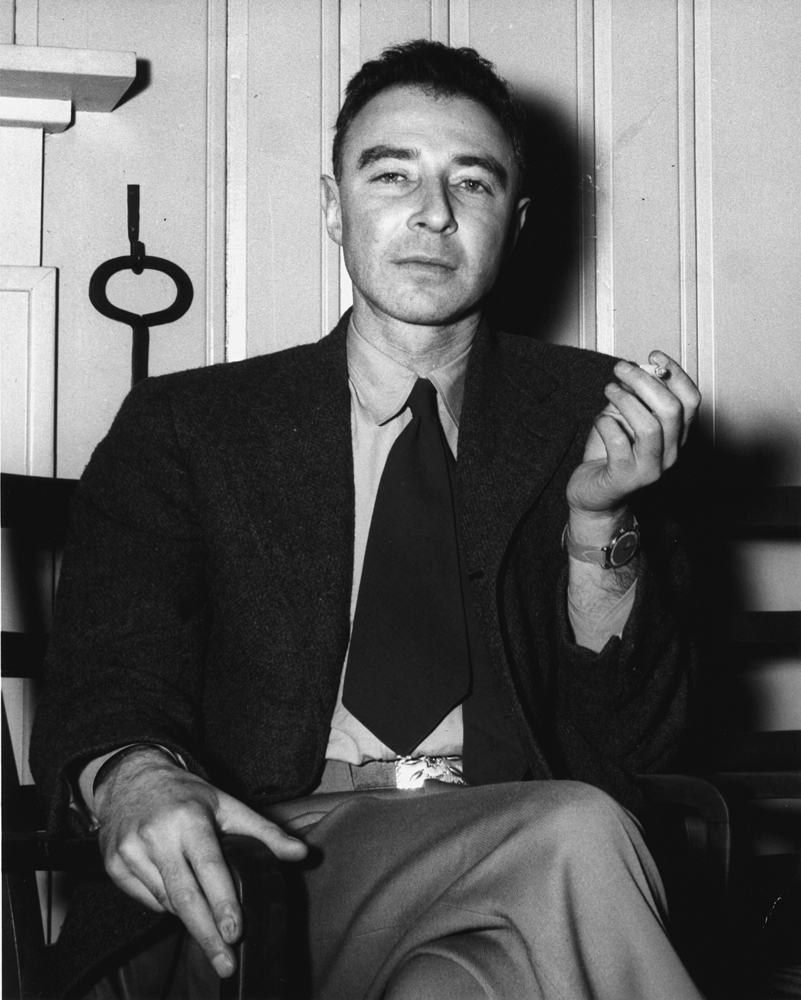
\includegraphics[keepaspectratio,width=0.5\linewidth]{oppenheimer}
\captionof{figure}{Relaxed atomic operations circa 1946}
\label{oppenheimer}
\end{colfigure}
This might seem like a rare occurrence,
but is surprisingly common.
Recall our examples from \secref{atomicity} and \secref{rmw} where some worker
thread increments a counter which is read by a \textsc{ui} thread to show
progress.
That counter could be incremented with
\texttt{atomic\_fetch\_add()} using \texttt{memory\_order\_relaxed}.
All we need is atomicity---nothing is synchronized by the counter.

Relaxed reads and writes are also useful for sharing flags between threads.
Consider some thread that loops until told to exit:
\begin{colfigure}
\begin{minted}[fontsize=\codesize]{cpp}
atomic_bool stop(false);

void worker()
{
  while (!stop.load(memory_order_relaxed)) {
    // Do good work.
  }
}

int main()
{
  launchWorker();
  // Wait some...
  stop = true; // seq_cst
  joinWorker();
}
\end{minted}
\end{colfigure}
We don't care if the contents of the loop are rearranged around the load.
Nothing bad will happen so long as \texttt{stop} only indicates that the
worker should exit and doesn't ``announce'' any new data to be
read by the worker.

Finally, relaxed loads are commonly used with \textsc{cas} loops.
Return to our lock-free multiply:
\begin{colfigure}
\begin{minted}[fontsize=\codesize]{cpp}
void atomicMultiply(int by)
{
  int expected = foo.load(memory_order_relaxed);

  while (!foo.compare_exchange_weak(
    expected, expected * by,
    memory_order_release,
    memory_order_relaxed))
  { /* empty loop */ }
}
\end{minted}
\end{colfigure}
All of the loads can be relaxed, as we don't need to enforce any sort of ordering
until we've successfully modified our value.
The initial load of \texttt{expected} isn't even strictly necessary---it just
saves us a loop iteration if no other thread modifies \texttt{foo} before the
\textsc{cas}.

\subsection{Acquire-Release}

\texttt{memory\_order\_acq\_rel} is used with atomic \textsc{rmw} operations
that need to both load-acquire \emph{and} store-release a value.
A typical example involves thread-safe reference counting,
like in \cpp{}'s \mintinline{cpp}{shared_ptr}:
\begin{colfigure}
\begin{minted}[fontsize=\codesize]{cpp}
atomic_int refCount;

void inc()
{
  refCount.fetch_add(1, memory_order_relaxed);
}
\end{minted}
\end{colfigure}
\begin{colfigure}
\begin{minted}[fontsize=\codesize]{cpp}
void dec()
{
  if (refCount.fetch_sub(1,
      memory_order_acq_rel) == 1) {
    // No more references, delete the data.
  }
}
\end{minted}
\end{colfigure}

Order doesn't matter when incrementing the reference
count since no action is taken as a result.
However, when we decrement, we must ensure that:
\begin{enumerate}
\item All reads and writes to the referenced object occur
\emph{before} the count reaches zero.
\item Deletion occurs \emph{after} the reference count drops to
    zero.\punckern\footnote{This can be optimized even further by
    making the acquire barrier only occur conditionally, when the reference
    count is zero.
    Standalone barriers are outside the scope of this paper,
    since they're almost always pessimal compared to a combined load-acquire
    or store-release, but you can see an example here:
    \url{http://www.boost.org/doc/libs/release/doc/html/atomic/usage\_examples.html}.}
\end{enumerate}

Curious readers might be wondering about the difference between
acquire-release and sequentially consistent operations.
To quote Hans Boehm, chair of the ISO~\cpp{} Concurrency Study Group,
\begin{quote}
\small
The difference between \texttt{acq\_rel} and \texttt{seq\_cst} is generally
whether the operation is required to participate in the
single global order of sequentially consistent operations.
\end{quote}
In other words, acquire-release provides order relative to the variable
being load-acquired and store-released, whereas sequentially consistent
operation provides some \emph{global} order across the entire program.
If the distinction still seems hazy, you're not alone.
Boehm continues with,
\begin{quote}
\small
This has subtle and unintuitive effects.
The [barriers] in the current standard may be the most
experts-only construct we have in the language.
\end{quote}

\subsection{Consume}

Last but not least, we have \texttt{memory\_order\_consume}.
Consider a scenario where data is rarely changed,
but frequently read by multiple threads.
Perhaps it is a pointer in the kernel to information about peripherals
plugged into the machine.
This data will change \emph{very} infrequently,
so it makes sense to optimize reads as much as possible.
Given what we know so far, the best we can do is:
\begin{colfigure}
\begin{minted}[fontsize=\codesize]{cpp}
std::atomic<PeripheralData*> peripherals;

// Writers:
PeripheralData* p = kAllocate(sizeof(*p));
populateWithNewDeviceData(p);
peripherals.store(p, memory_order_release);
\end{minted}
\begin{minted}[fontsize=\codesize]{cpp}
// Readers:
PeripheralData* p =
    peripherals.load(memory_order_acquire);
if (p != nullptr) {
    doSomethingWith(p->keyboards);
}
\end{minted}
\end{colfigure}

Since we want to optimize readers as much as possible,
it would be quite nice if we could avoid a memory barrier
on weakly-ordered systems.
As it turns out, we usually can.
Since the data we examine (\texttt{p->keyboards})
is \emph{dependent} on the value of \texttt{p},
most platforms---even weakly-ordered ones---cannot reorder the initial
load (\mintinline{cpp}{p = peripherals}) to take place after its use
(\mintinline{cpp}{p->keyboards}).\punckern\footnote{Much to everybody's chagrin,
this \emph{isn't} the case on some extremely weakly-ordered architectures like
DEC Alpha.}
So long as we convince the compiler not to make any similar speculations,
we're in the clear.
This is what \monobox{memory\_order\_consume} is for.
Change readers to:
\begin{colfigure}
\begin{minted}[fontsize=\codesize]{cpp}
PeripheralData* p =
    peripherals.load(memory_order_consume);
if (p != nullptr) {
    doSomethingWith(p->keyboards);
}
\end{minted}
\end{colfigure}
and an \textsc{arm} compiler could emit:
\begin{colfigure}
\begin{lstlisting}[language={[ARM]Assembler}]
  ldr r3, &peripherals
  ldr r3, [r3]
  // Look ma, no barrier!
  cbz r3, was_null // Check for null
  ldr r0, [r3, #4] // Load p->keyboards
  b doSomethingWith(Keyboards*)
was_null:
  ...
\end{lstlisting}
\end{colfigure}

Sadly, the emphasis here is on \emph{could.}
Figuring out what constitutes a ``dependency'' between expressions isn't
as trivial as one might hope,\punckern\footnote{Even the experts in
the \textsc{iso} committee's concurrency study group, \textsc{sg}1,
came away with different understandings.
See
\href{http://www.open-std.org/jtc1/sc22/wg21/docs/papers/2014/n4036.pdf}{\textsc{n}4036}
for the gory details.
Proposed solutions are explored in
\href{http://www.open-std.org/jtc1/sc22/wg21/docs/papers/2017/p0190r3.pdf}{\textsc{p}0190\textsc{r}3}
and
\href{http://www.open-std.org/jtc1/sc22/wg21/docs/papers/2017/p0462r1.pdf}{\textsc{p}0462\textsc{R}1}.
}
so all compilers currently convert consume operations to acquires.

\subsection{\textsc{Hc Svnt Dracones}}

Non-sequentially consistent orderings have many subtleties,
and a slight mistake can cause elusive Heisenbugs that only occur sometimes,
on some platforms.
Before reaching for them, ask yourself:
\begin{itemize}[label={}, before=\itshape]
\item Am I using a well-known and understood pattern \\
      (such as the ones shown above)?
\item Are the operations in a tight loop?
\item Does every microsecond count here?
\end{itemize}
If the answer isn't yes for at least one of these,
default to sequentially consistent operations.
Otherwise, be sure to give your code extra review and testing.

\section{Hardware convergence}

Those familiar with the platform may have noticed that all \textsc{arm} assembly
shown here is from the seventh version of the architecture.
Excitingly, the current (eighth) generation offers a massive
improvement for lockless code.
Since most programming languages have converged on the memory model we've been
exploring, \textsc{arm}v8 processors offer dedicated load-acquire
and store-release instructions, \keyword{lda} and \keyword{stl}.
We can use them to implement everything we've discussed here without
resorting to memory barriers.
Hopefully, future \textsc{cpu} architectures will follow suit.

\section{If concurrency is the question, \texttt{volatile} is not the answer.}

Before we go, we should lay a common misconception surrounding
the \keyword{volatile} keyword to rest.
Perhaps because of how it worked in older compilers and hardware,
or because of its different meaning in languages like
Java and \csharp,\punckern\footnote{Unlike in \clang{} and \cpp{},
\keyword{volatile} \emph{does} enforce ordering in those languages.}
some believe that the keyword is useful for building concurrency tools.
Except for one specific case (see \secref{fusing}), this is false.

The purpose of \keyword{volatile} is to inform the compiler that a value can
be changed by something besides the program we're executing.
This is useful for memory-mapped~\textsc{I/O} \textsc{(mmio)},
where the system hardware translates reads and writes to certain addresses
into instructions for the devices connected to the \textsc{cpu}.
(This is how most machines ultimately interact with the outside world.)
This implies two guarantees:
\begin{enumerate}
\item The compiler will not elide what it would otherwise see as ``unnecessary''
    loads and stores. For example, if I had some function:
    \begin{colfigure}
    \begin{minted}[fontsize=\codesize,autogobble]{cpp}
    void write(int* t)
    {
      *t = 2;
      *t = 42;
    }
    \end{minted}
    \end{colfigure}
    the compiler would normally optimize it to:
    \begin{minted}[fontsize=\codesize,autogobble]{cpp}
    void write(int* t) { *t = 42; }
    \end{minted}
    \mintinline{cpp}{*t = 2} is usually assumed to be a
    \introduce{dead store} with no effect.
    But, if \texttt{t} points to some \textsc{mmio} register, it's not
    safe to make this assumption---each write could have some effect
    on the hardware it's interacting with.

\item The compiler will not reorder \keyword{volatile}
    reads and writes with respect to other \keyword{volatile} ones
    for similar reasons.
\end{enumerate}

These don't give us the atomicity or order we need for safe
inter-thread communication.
Notice that the second guarantee only prevents \keyword{volatile} operations
from being reordered in relation \emph{to each other}---the compiler is still
free to rearrange all other ``normal'' loads and stores around them.
And even if we got past that problem, \keyword{volatile} does not emit memory
barriers on weakly-ordered hardware.
The keyword only works as a synchronization mechanism if both your compiler
\emph{and} your hardware perform no reodrering.
Don't bet on that.

\section{Optimizations}
\label{fusing}

Finally, one should realize that while atomic operations do prevent certain
optimizations, they aren't somehow immune to all of them.
The optimizer can do fairly mundane things, such as replacing
\monobox{foo.fetch\_and(0)} with \monobox{foo = 0},
but it can also produce surprising results.
Consider:
\begin{colfigure}
\begin{minted}[fontsize=\codesize]{cpp}
while (tmp = foo.load(memory_order_relaxed)) {
  doSomething(tmp);
}
\end{minted}
\end{colfigure}
Since relaxed loads provide no ordering guarantees,
the compiler is free to unroll the loop as much as it pleases,
perhaps into:
\begin{colfigure}
\begin{minted}[fontsize=\codesize]{cpp}
while (tmp = foo.load(memory_order_relaxed)) {
  doSomething(tmp);
  doSomething(tmp);
  doSomething(tmp);
  doSomething(tmp);
}
\end{minted}
\end{colfigure}
In some cases, ``fusing'' reads or writes like this is unacceptable,
so we must prevent it
with \mintinline{cpp}{volatile} casts or incantations like
\mintinline{cpp}{asm volatile("" ::: "memory")}.\punckern\footnote{See
\url{https://stackoverflow.com/a/14983432}.}
The Linux kernel provides \monobox{READ\_ONCE()} and \monobox{WRITE\_ONCE()}
macros for this exact purpose.\punckern\footnote{See
\href{http://www.open-std.org/jtc1/sc22/wg21/docs/papers/2015/n4374.html}{\textsc{n}4374}
and the kernel's
\href{http://elixir.free-electrons.com/linux/latest/source/include/linux/compiler.h}{\texttt{compiler.h}}
for details.}

\section{Takeaways}

We've only scratched the surface here,
but hopefully you now know:
\begin{itemize}
\item Why compilers and \textsc{cpu} hardware reorder loads and stores.
\item Why we need special tools to prevent these reorderings
    to communicate between threads.
\item How we can guarantee \introduce{sequential consistency} in our programs.
\item Atomic \introduce{read-modify-write} operations.
\item How atomic operations can be implemented on weakly-ordered hardware,
    and what implications this can have for a language-level \textsc{api}.
\item How we can \emph{carefully} optimize lockless code using alternative
    memory orderings.
\item Why \keyword{volatile} is an inappropriate tool for inter-thread
    communication.
\item How the compiler might optimize atomic operations even further,
    and what we can do to prevent certain undesirable optimizations.
\end{itemize}
To learn more, see the additional resources below,
or examine lock-free data structures and algorithms,
such as a \introduce{single-producer/single-consumer}
\textsc{(sp/sc)} queue or \introduce{read-copy-update}
\textsc{(rcu)}.\punckern\footnote{See the Linux Weekly News article,
\href{https://lwn.net/Articles/262464/}{\textit{What is RCU, Fundamentally?}}
for an introduction.}

\vspace{\baselineskip}
\noindent Good luck and godspeed!

\end{multicols*}

\appendix
\setcounter{secnumdepth}{0}

\begin{center}
\begin{minipage}{0.7\linewidth}
\setlength\parskip{\baselineskip}
\setlength\parindent{0pt}
\section{Additional Resources}

\href{https://www.youtube.com/watch?v=ZQFzMfHIxng}{%
\textit{\cpp{} atomics, from basic to advanced. What do they really do?}}
by Fedor Pikus,
a hour-long talk on this topic.

\href{https://channel9.msdn.com/Shows/Going+Deep/Cpp-and-Beyond-2012-Herb-Sutter-atomic-Weapons-1-of-2}{%
\textit{\texttt{atomic<> Weapons}: The \cpp{11} Memory Model and Modern Hardware}}
by Herb Sutter,
a three-hour talk that provides
a deeper dive.
Also the source of figures
\ref{ideal-machine} and \ref{dunnington}.

\href{https://www.akkadia.org/drepper/futex.pdf}{\textit{Futexes are Tricky}},
a paper by Ulrich Drepper on how mutexes and other synchronization primitives
can be built in Linux using atomic operations and syscalls.

\href{https://www.kernel.org/pub/linux/kernel/people/paulmck/perfbook/perfbook.html}{%
\textit{Is Parallel Programming Hard, And, If So, What Can You Do About It?}},
by Paul~E.\ McKenney,
an \emph{incredibly} comprehensive book covering parallel data structures and
algorithms, transactional memory, cache coherence protocols,
\textsc{cpu} architecture specifics, and more.

\href{http://www.rdrop.com/~paulmck/scalability/paper/whymb.2010.06.07c.pdf}{%
\textit{Memory Barriers: a Hardware View for Software Hackers}},
an older but much shorter piece by McKenney explaining how memory barriers are implemented
in the Linux kernel on various architectures.

\href{http://preshing.com/archives/}{\textit{Preshing On Programming}},
a blog with many excellent articles on lockless concurrency.

\textit{No Sane Compiler Would Optimize Atomics}, a discussion of how
atomic operations are handled by current optimizers.
Available as a writeup,
\href{http://www.open-std.org/jtc1/sc22/wg21/docs/papers/2015/n4455.html}{%
\textsc{n}4455}, and as a
\href{https://www.youtube.com/watch?v=IB57wIf9W1k}{CppCon talk}.

\href{http://en.cppreference.com}{cppreference.com},
an excellent reference for the \clang{} and \cpp{} memory model and
atomic \textsc{api}.

\href{https://godbolt.org/}{Matt Godbolt's Compiler Explorer},
an online tool that provides live, color-coded disassembly using compilers and
flags of your choosing.
\emph{Fantastic} for examining what compilers emit for various
atomic operations on different architectures.

\section{About This Document}

\subsection{Contributing}

Contributions are welcome!
Sources and history are available on
\href{https://gitlab.com/mrkline/lockless-concurrency}{Gitlab}
and
\href{https://github.com/mrkline/lockless-concurrency}{Github}.
This paper is prepared in \LaTeX{}---if you're not familiar with it,
feel free to contact the author
(via email, by opening an issue, etc.)
in lieu of pull requests.

\subsection{License}

\addfontfeature{Numbers=LowercaseOff}
This paper is licensed under a
Creative Commons Attribution-ShareAlike 4.0 International License.
The legalese can be found through
\url{https://creativecommons.org/licenses/by-sa/4.0/},
but in short,
you are free to copy, redistribute, translate, or otherwise transform this paper
so long as you give appropriate credit, indicate if changes were made,
and release your version or copy under this same license.

\end{minipage}
\end{center}

\end{document}
